\ifdefined\inMainDoc\else
\documentclass[12pt,a4paper]{article}
% ================================================================
%  PRÉAMBULE COMMUN - ANNALES CORRIGÉES
%  Université de Kara - FaST - Licence Fondamentale MPC
%  Design optimisé impression noir et blanc
% ================================================================

% -- ENCODAGE & LANGUE --
\usepackage[utf8]{inputenc}
\usepackage[T1]{fontenc}
\usepackage[french]{babel}
\usepackage{lmodern}
\usepackage{microtype}

% -- MISE EN PAGE --
\usepackage[a4paper, top=2.8cm, bottom=2.5cm, left=2.5cm, right=2.5cm, headheight=14pt]{geometry}
\usepackage{setspace}
\setstretch{1.2}
\usepackage{parskip}
\setlength{\parindent}{1.2em}
\setlength{\parskip}{4pt}

% -- MATHS --
\usepackage{amsmath, amssymb, mathtools, amsthm}
\usepackage{mathrsfs}
\usepackage{dsfont}
\usepackage{bm}
\usepackage{cancel}
\usepackage{textcomp}
% Définition de \oiint (intégrale de surface fermée) sans package supplémentaire
\newcommand{\oiint}{\mathop{\iint\!\!\!\!\!\!\!\bigcirc}\limits}

% -- PHYSIQUE & CHIMIE --
\usepackage{physics}
\usepackage{siunitx}
% Lorsque physics est chargé, siunitx omet \qty. On le restaure ici :
\AtBeginDocument{\RenewCommandCopy\qty\SI}
\sisetup{locale = FR, detect-all, output-decimal-marker={,}}
% Commande de substitution pour les unités posant problème avec pdflatex
% (ohm, degreeCelsius, micro, angstrom, percent utilisent des caractères non-ASCII)
\newcommand{\qtyohm}[1]{\ensuremath{\num{#1}\,\Omega}}
\newcommand{\qtydegc}[1]{\ensuremath{\num{#1}\,{}^\circ\text{C}}}
\newcommand{\qtyangstrom}[1]{\ensuremath{\num{#1}\,\text{\AA}}}
\newcommand{\qtypercent}[1]{\ensuremath{\num{#1}\,\%}}
\newcommand{\qtyum}[1]{\ensuremath{\num{#1}\,\mu\text{m}}}
\usepackage[version=4]{mhchem}

% -- GRAPHISMES --
\usepackage{graphicx}
\usepackage{float}
\usepackage{caption}
\usepackage{subcaption}
\usepackage{wrapfig}
\usepackage{tikz}
\usetikzlibrary{calc, arrows.meta, patterns, shapes.geometric}
\usepackage{pgfplots}
\pgfplotsset{compat=1.18}

% -- TABLEAUX --
\usepackage{booktabs}
\usepackage{array}
\usepackage{tabularx}
\usepackage{multirow}

% -- LISTES --
\usepackage{enumitem}
\setlist[enumerate]{topsep=3pt, itemsep=2pt, parsep=0pt}
\setlist[itemize]{topsep=3pt, itemsep=2pt, parsep=0pt, label={.}}

% -- BOÎTES (noir et blanc) --
\usepackage{mdframed}
\usepackage{tcolorbox}
\tcbuselibrary{skins, breakable, theorems}

% Boîte EXERCICE : encadré avec filet épais, fond blanc
\newmdenv[
  linewidth=1.2pt,
  linecolor=black,
  roundcorner=3pt,
  skipabove=10pt,
  skipbelow=6pt,
  innertopmargin=8pt,
  innerbottommargin=8pt,
  innerleftmargin=10pt,
  innerrightmargin=10pt,
  backgroundcolor=white,
  frametitle={\bfseries\small Exercice},
  frametitlealignment=\raggedright,
  frametitleaboveskip=4pt,
  frametitlebelowskip=4pt,
]{boiteexercice}

% Boîte CORRIGÉ : fond gris très clair + filet fin
\newmdenv[
  linewidth=0.6pt,
  linecolor=black,
  leftline=true,
  rightline=false,
  topline=false,
  bottomline=false,
  linecolor=black,
  innerleftmargin=12pt,
  innerrightmargin=8pt,
  innertopmargin=6pt,
  innerbottommargin=6pt,
  backgroundcolor=gray!8,
  skipabove=4pt,
  skipbelow=8pt,
]{boitecorrige}

% Boîte RÉSUMÉ DE COURS : double encadré
\newmdenv[
  linewidth=0.8pt,
  linecolor=black,
  roundcorner=2pt,
  backgroundcolor=gray!12,
  innertopmargin=10pt,
  innerbottommargin=10pt,
  innerleftmargin=12pt,
  innerrightmargin=12pt,
  skipabove=12pt,
  skipbelow=8pt,
]{boiteresume}

% Boîte ATTENTION/REMARQUE : barre gauche épaisse
\newmdenv[
  leftline=true,
  rightline=false,
  topline=false,
  bottomline=false,
  linewidth=3pt,
  linecolor=black,
  backgroundcolor=gray!5,
  innerleftmargin=12pt,
  innerrightmargin=8pt,
  innertopmargin=5pt,
  innerbottommargin=5pt,
  skipabove=6pt,
  skipbelow=6pt,
]{boiteremarque}

% -- DIFFICULTÉ DES EXERCICES --
\newcommand{\facile}{$\star$}
\newcommand{\moyen}{$\star\!\star$}
\newcommand{\difficile}{$\star\!\star\!\star$}
\newcommand{\niveau}[1]{\hfill\textbf{#1}\hspace{2pt}}

% -- EN-TÊTES ET PIEDS DE PAGE --
\usepackage{fancyhdr}
\pagestyle{fancy}
\fancyhf{}
\renewcommand{\headrulewidth}{0.5pt}
\renewcommand{\footrulewidth}{0.3pt}

% -- HYPERLIENS --
\usepackage[hidelinks]{hyperref}
\hypersetup{
    colorlinks=false,
    pdftitle={Annale Corrigée - Licence MPC - Université de Kara}
}

% -- TITRES --
\usepackage{titlesec}
\titleformat{\section}{\Large\bfseries}{\thesection.}{0.8em}{}[\vspace{2pt}\hrule\vspace{4pt}]
\titleformat{\subsection}{\large\bfseries}{\thesubsection.}{0.7em}{}
\titleformat{\subsubsection}{\normalsize\bfseries}{\thesubsubsection.}{0.6em}{}

% -- THÉORÈMES --
\theoremstyle{definition}
\newtheorem{defn}{Définition}[section]
\newtheorem{prop}{Propriété}[section]
\newtheorem{thm}{Théorème}[section]
\newtheorem{corol}{Corollaire}[section]
\newtheorem{exemple}{Exemple}[section]

% -- COMMANDES MATHÉMATIQUES UTILES --
\newcommand{\vect}[1]{\overrightarrow{#1}}
\newcommand{\R}{\mathbb{R}}
\newcommand{\N}{\mathbb{N}}
\newcommand{\Z}{\mathbb{Z}}
\newcommand{\C}{\mathbb{C}}
\renewcommand{\d}{\mathrm{d}}
\newcommand{\deriv}[2]{\dfrac{\d #1}{\d #2}}
\newcommand{\dpart}[2]{\dfrac{\partial #1}{\partial #2}}
\newcommand{\rot}{\overrightarrow{\mathrm{rot}}\,}
\renewcommand{\div}{\mathrm{div}\,}
\renewcommand{\grad}{\overrightarrow{\mathrm{grad}}\,}
\newcommand{\e}{\mathrm{e}}
\newcommand{\ii}{\mathrm{i}}
\renewcommand{\Tr}{\mathrm{Tr}}

% Numérotation des équations par section
\numberwithin{equation}{section}

% -- RÉSULTATS ENCADRÉS --
\newcommand{\res}[1]{\[\boxed{#1}\]}

% -- REMARQUE INLINE --
\newcommand{\rmq}[1]{\begin{boiteremarque}\textbf{Remarque.} #1\end{boiteremarque}}

% -- MISE EN VALEUR DU RÉSULTAT FINAL --
\newcommand{\reponse}[1]{%
  \begin{center}
    \fbox{\begin{minipage}{0.92\textwidth}\centering #1\end{minipage}}
  \end{center}%
}


\lhead{\small\textit{Propagation des Ondes - Licence 3}}
\rhead{\small\textit{FaST, Université de Kara}}
\cfoot{\thepage}

\begin{document}
\fi

\begin{center}
  {\LARGE\bfseries PROPAGATION DES ONDES ÉLECTROMAGNÉTIQUES}\\[0.3cm]
  {\normalsize Licence 3 - Physique}\\[0.1cm]
  \rule{0.7\textwidth}{0.8pt}
\end{center}

\section*{Résumé du cours}

\begin{boiteresume}

\textbf{1. Équations de Maxwell dans le vide.} En l'absence de charges et de courants libres :
\[
\mathrm{div}\,\vec{E}=0,\quad \mathrm{div}\,\vec{B}=0,\quad \overrightarrow{\mathrm{rot}}\,\vec{E}=-\frac{\partial\vec{B}}{\partial t},\quad \overrightarrow{\mathrm{rot}}\,\vec{B}=\mu_0\varepsilon_0\frac{\partial\vec{E}}{\partial t}
\]

\textbf{2. Équation de propagation.} En combinant Maxwell-Faraday et Maxwell-Ampère : $\Delta\vec{E}-\frac{1}{c^2}\frac{\partial^2\vec{E}}{\partial t^2}=\vec{0}$ avec $c=1/\sqrt{\mu_0\varepsilon_0}$.

\textbf{3. Onde plane progressive harmonique (OPPH).} Solution : $\vec{E} = \vec{E}_0\,\e^{\ii(\omega t - \vec{k}\cdot\vec{r})}$. Le vecteur d'onde $\vec{k}$ est la direction de propagation, $k = \omega/c$. Structure transversale : $\vec{E}\perp\vec{B}\perp\vec{k}$ (trièdre direct). Relation : $\vec{B} = \frac{1}{c}\hat{k}\wedge\vec{E}$.

\textbf{4. Impédance et rapport de champs.} $Z_0 = \sqrt{\mu_0/\varepsilon_0} \approx \qty{377}{\Omega}$ est l'impédance du vide. $E/B = c$, $E/H = Z_0$.

\textbf{5. Vecteur de Poynting.} $\vec{\Pi} = \vec{E}\wedge\vec{H} = \frac{1}{\mu_0}\vec{E}\wedge\vec{B}$. C'est la densité de flux d'énergie (W/m²). Valeur moyenne : $\langle\Pi\rangle = \frac{E_0^2}{2Z_0}$.

\textbf{6. Propagation dans un milieu.} Dans un milieu linéaire, isotrope, homogène (LIH) de permittivité $\varepsilon_r$ et perméabilité $\mu_r$ : $v = c/n$ avec $n=\sqrt{\varepsilon_r\mu_r}$ l'indice optique. Relation de dispersion : $k = n\omega/c$.

\textbf{7. Vitesses.} Vitesse de phase : $v_\phi = \omega/k$. Vitesse de groupe : $v_g = \mathrm{d}\omega/\mathrm{d}k$. Dans le vide : $v_\phi = v_g = c$.

\end{boiteresume}

\newpage
\section{Ondes planes dans le vide}

\subsection*{Exercice 1 - Structure d'une onde plane \niveau{\facile}}

\begin{boiteexercice}
Soit le champ magnétique d'une onde plane sinusoïdale se propageant dans le vide :
\[
\vec{H}(y,t) = H_0\sin(\omega t - \beta y)\,\vec{u}_z
\]
\begin{enumerate}
  \item Indiquer la direction de propagation et le plan de polarisation.
  \item Calculer le champ électrique $\vec{E}(y,t)$ en utilisant la relation de Maxwell-Faraday.
  \item Vérifier le résultat en utilisant la relation $\vec{E} = Z_0\,\vec{H}\wedge\hat{u}_y$.
  \item Calculer le vecteur de Poynting instantané et sa valeur moyenne.
\end{enumerate}
\end{boiteexercice}

\begin{boitecorrige}
\textbf{1.} Le vecteur d'onde est $\vec{k} = \beta\,\vec{u}_y$, donc la propagation est suivant $Oy$. Le champ $\vec{H}$ est selon $\vec{u}_z$, donc le plan de polarisation est le plan $Oyz$.

\textbf{2.} Maxwell-Faraday : $\overrightarrow{\mathrm{rot}}\,\vec{E} = -\mu_0\frac{\partial\vec{H}}{\partial t}$. L'onde se propageant suivant $y$, $\vec{E}$ dépend seulement de $y$ et $t$. L'équation selon $\vec{u}_z$ donne :
\[
-\frac{\partial E_x}{\partial y} = -\mu_0\frac{\partial H_z}{\partial t} = -\mu_0\omega H_0\cos(\omega t-\beta y)
\]
En intégrant en $y$ :
\[
E_x = \frac{\mu_0\omega}{\beta}H_0\sin(\omega t-\beta y) = \frac{\mu_0 c}{1} H_0\sin(\omega t-\beta y) = Z_0 H_0\sin(\omega t-\beta y)
\]
(car $\beta = \omega/c$ et $Z_0 = \mu_0 c$). Donc :
\[
\vec{E}(y,t) = Z_0 H_0\sin(\omega t-\beta y)\,\vec{u}_x
\]

\textbf{3.} Vérification : $\vec{H}\wedge\hat{u}_y = H_0\sin(\omega t-\beta y)(\vec{u}_z\wedge\vec{u}_y) = -H_0\sin(\omega t-\beta y)\,\vec{u}_x$. Le signe est cohérent avec $\vec{E} = -Z_0(\vec{H}\wedge\hat{u}_y)$ pour une propagation en $+y$ (trièdre direct $\vec{E},\vec{H},\hat{k}$). On retrouve bien $E_x = Z_0 H_0\sin(\omega t-\beta y)$.

\textbf{4.} Vecteur de Poynting : $\vec{\Pi} = \vec{E}\wedge\vec{H}$. $\vec{E} = E_x\vec{u}_x$, $\vec{H} = H_z\vec{u}_z$ donc :
\[
\vec{\Pi} = E_x H_z\,(\vec{u}_x\wedge\vec{u}_z) = -E_x H_z\,\vec{u}_y
\]
Avec $E_x = Z_0 H_0\sin(\omega t-\beta y)$ et $H_z = H_0\sin(\omega t-\beta y)$ :
\[
\vec{\Pi} = -Z_0 H_0^2\sin^2(\omega t-\beta y)\,\vec{u}_y
\]
Valeur moyenne ($\langle\sin^2\rangle = 1/2$) : $\langle\vec{\Pi}\rangle = -\frac{Z_0 H_0^2}{2}\,\vec{u}_y$.

Le signe négatif vient du choix de $\vec{H}$ selon $+\vec{u}_z$, donnant une propagation en $-y$. La puissance transportée est $|\langle\Pi\rangle| = Z_0 H_0^2/2$.
\end{boitecorrige}

\subsection*{Exercice 2 - Équation de propagation et solution générale \niveau{\moyen}}

\begin{boiteexercice}
\begin{enumerate}
  \item À partir des équations de Maxwell dans le vide, établir l'équation de propagation de $\vec{E}$.
  \item Montrer qu'une fonction de la forme $f(z,t) = f_1(t-z/c) + f_2(t+z/c)$ est solution de l'équation de propagation scalaire.
  \item Pour $\vec{E} = E_0\cos(\omega t - kz)\,\vec{e}_x$ :
  \begin{enumerate}[label=(\alph*)]
    \item Vérifier que $\vec{E}$ satisfait l'équation de propagation.
    \item Trouver $\vec{B}$ associé à partir de Maxwell-Faraday.
    \item Décrire la nature du trièdre $(\vec{E},\vec{B},\vec{k})$.
  \end{enumerate}
  \item Déterminer la relation de dispersion. Le vide est-il dispersif ?
  \item Calculer les vitesses de phase et de groupe.
\end{enumerate}
\end{boiteexercice}

\begin{boitecorrige}
\textbf{1.} On applique $\overrightarrow{\mathrm{rot}}$ à Maxwell-Faraday et on utilise l'identité vectorielle $\overrightarrow{\mathrm{rot}}(\overrightarrow{\mathrm{rot}}\,\vec{E}) = \overrightarrow{\mathrm{grad}}(\mathrm{div}\,\vec{E}) - \Delta\vec{E} = -\Delta\vec{E}$ (car $\mathrm{div}\,\vec{E}=0$) :
\[
-\Delta\vec{E} = \overrightarrow{\mathrm{rot}}\!\left(-\frac{\partial\vec{B}}{\partial t}\right) = -\frac{\partial}{\partial t}(\overrightarrow{\mathrm{rot}}\,\vec{B}) = -\mu_0\varepsilon_0\frac{\partial^2\vec{E}}{\partial t^2}
\]
D'où l'équation de propagation (ou équation d'onde) :
\[
\boxed{\Delta\vec{E} - \frac{1}{c^2}\frac{\partial^2\vec{E}}{\partial t^2} = \vec{0}}
\]

\textbf{2.} Pour $f(z,t) = f_1(t-z/c)+f_2(t+z/c)$, on calcule :
\[
\frac{\partial^2 f}{\partial z^2} = \frac{1}{c^2}f_1'' + \frac{1}{c^2}f_2'' = \frac{1}{c^2}\frac{\partial^2 f}{\partial t^2}
\]
donc $\partial^2 f/\partial z^2 - (1/c^2)\partial^2 f/\partial t^2 = 0$ : $f$ est bien solution. $f_1$ représente une onde progressant en $+z$ et $f_2$ en $-z$.

\textbf{3a.} Pour $E_x = E_0\cos(\omega t - kz)$ :
\[
\frac{\partial^2 E_x}{\partial z^2} = -k^2 E_x, \qquad \frac{\partial^2 E_x}{\partial t^2} = -\omega^2 E_x
\]
L'équation de propagation donne $-k^2 + \omega^2/c^2 = 0$, soit $k = \omega/c$ : vérifiée.

\textbf{3b.} Maxwell-Faraday : $\partial B_y/\partial t = \partial E_x/\partial z$. Donc :
\[
B_y = \frac{k}{\omega}E_0\sin(\omega t-kz) = \frac{E_0}{c}\sin(\omega t-kz)
\]

Plus précisément, Maxwell-Faraday donne :
\[
(\overrightarrow{\mathrm{rot}}\,\vec{E})_y = -\frac{\partial E_x}{\partial z} = kE_0\sin(\omega t-kz) = -\frac{\partial B_y}{\partial t}
\]
\[
\Rightarrow B_y = \frac{k}{\omega}E_0\cos(\omega t-kz) = \frac{E_0}{c}\cos(\omega t-kz)
\]
Donc $\vec{B} = \frac{E_0}{c}\cos(\omega t-kz)\,\vec{e}_y$.

\textbf{3c.} $\vec{E}\parallel\vec{e}_x$, $\vec{B}\parallel\vec{e}_y$, $\vec{k}\parallel\vec{e}_z$ : ils forment un \textbf{trièdre direct orthogonal}. L'onde est transversale ($\vec{E}$ et $\vec{B}$ perpendiculaires à la direction de propagation).

\textbf{4.} La relation de dispersion $k = \omega/c$ est \textbf{linéaire} : le vide n'est \textbf{pas dispersif}.

\textbf{5.} $v_\phi = \omega/k = c$ et $v_g = \mathrm{d}\omega/\mathrm{d}k = c$. Les deux vitesses sont égales à $c \approx \qty{3e8}{m.s^{-1}}$.
\end{boitecorrige}

\subsection*{Exercice 3 - Bilan énergétique \niveau{\moyen}}

\begin{boiteexercice}
Pour une OPPH se propageant dans le vide : $\vec{E} = E_0\cos(\omega t - kz)\,\vec{e}_x$.
\begin{enumerate}
  \item Exprimer la densité d'énergie électromagnétique $u_{em} = \frac{\varepsilon_0 E^2}{2} + \frac{B^2}{2\mu_0}$.
  \item Calculer la valeur moyenne temporelle $\langle u_{em}\rangle$.
  \item Calculer le vecteur de Poynting $\vec{\Pi} = \frac{1}{\mu_0}\vec{E}\wedge\vec{B}$ et sa valeur moyenne.
  \item Vérifier la relation $\langle\Pi\rangle = c\langle u_{em}\rangle$ (énergie transportée à la vitesse $c$).
  \item Écrire l'équation locale de conservation de l'énergie.
\end{enumerate}
\end{boiteexercice}

\begin{boitecorrige}
On a $\vec{E} = E_0\cos(\omega t-kz)\,\vec{e}_x$ et $\vec{B} = (E_0/c)\cos(\omega t-kz)\,\vec{e}_y$.

\textbf{1.} Densité d'énergie :
\[
u_{em} = \frac{\varepsilon_0 E_0^2\cos^2(\omega t-kz)}{2} + \frac{E_0^2\cos^2(\omega t-kz)}{2\mu_0 c^2}
\]
Comme $\mu_0\varepsilon_0 c^2 = 1$, les deux termes sont égaux :
\[
u_{em} = \varepsilon_0 E_0^2\cos^2(\omega t-kz)
\]

\textbf{2.} $\langle u_{em}\rangle = \varepsilon_0 E_0^2/2$.

\textbf{3.} Vecteur de Poynting :
\[
\vec{\Pi} = \frac{1}{\mu_0}(E_0\vec{e}_x)\wedge\frac{E_0}{c}(\vec{e}_y)\cos^2(\omega t-kz) = \frac{E_0^2}{\mu_0 c}\cos^2(\omega t-kz)\,\vec{e}_z
\]
Valeur moyenne : $\langle\Pi\rangle = \frac{E_0^2}{2\mu_0 c} = \frac{\varepsilon_0 cE_0^2}{2} = c\langle u_{em}\rangle$

\textbf{4.} $\langle\Pi\rangle = \frac{E_0^2}{2Z_0}$ avec $Z_0 = \mu_0 c \approx \qty{377}{\Omega}$.

On vérifie $c\langle u_{em}\rangle = c\cdot\frac{\varepsilon_0 E_0^2}{2} = \frac{E_0^2}{2\mu_0 c} = \langle\Pi\rangle$ : l'énergie est bien transportée à la vitesse $c$.

\textbf{5.} Équation locale de conservation de l'énergie (théorème de Poynting) :
\[
\frac{\partial u_{em}}{\partial t} + \mathrm{div}\,\vec{\Pi} = 0
\]
(en l'absence de charges et de courants, il n'y a pas de dissipation).
\end{boitecorrige}

\section{Propagation dans un milieu}

\subsection*{Exercice 4 - Propagation dans un diélectrique \niveau{\moyen}}

\begin{boiteexercice}
Un diélectrique parfait a une permittivité relative $\varepsilon_r = 4$ et une perméabilité $\mu_r = 1$.
\begin{enumerate}
  \item Calculer l'indice optique $n$ et la vitesse de phase $v$ de l'onde dans ce milieu.
  \item Quelle est l'impédance caractéristique du milieu $Z = Z_0/n$ ?
  \item Une onde plane de fréquence $f = \qty{1}{GHz}$ ($\lambda_0 = \qty{30}{cm}$ dans le vide) se propage dans ce milieu. Calculer la longueur d'onde $\lambda$ dans le diélectrique.
  \item Quelle est la relation de dispersion ? Le milieu est-il dispersif (si $\varepsilon_r$ est indépendant de $\omega$) ?
\end{enumerate}
\end{boiteexercice}

\begin{boitecorrige}
\textbf{1.} $n = \sqrt{\varepsilon_r\mu_r} = \sqrt{4\times1} = 2$. Vitesse de phase : $v = c/n = \qty{3e8}{m.s^{-1}}/2 = \qty{1.5e8}{m.s^{-1}}$.

\textbf{2.} Impédance : $Z = Z_0/n = 377/2 \approx \qty{188.5}{\Omega}$.

\textbf{3.} Longueur d'onde : $\lambda = \lambda_0/n = \qty{30}{cm}/2 = \qty{15}{cm}$.

\textbf{4.} La relation de dispersion dans le diélectrique : $k = n\omega/c$. Si $\varepsilon_r$ est indépendant de $\omega$ (ce qui est une approximation), $n$ est constant et $k\propto\omega$ : la relation est linéaire, le milieu est \textbf{non dispersif}. En pratique, $\varepsilon_r$ dépend de $\omega$, ce qui introduit de la dispersion.
\end{boitecorrige}

\subsection*{Exercice 5 - Réflexion et transmission à une interface \niveau{\difficile}}

\begin{boiteexercice}
Une onde plane se propage dans le vide (milieu 1, $n_1=1$) et arrive en incidence normale sur une interface plane séparant le vide d'un diélectrique ($n_2=1{,}5$, comme le verre).

Les coefficients de Fresnel en incidence normale sont :
\[
r = \frac{n_1-n_2}{n_1+n_2}, \qquad t = \frac{2n_1}{n_1+n_2}
\]
et les coefficients de réflexion et de transmission en puissance sont $R = r^2$ et $T = \frac{n_2}{n_1}t^2$.
\begin{enumerate}
  \item Calculer $r$ et $t$.
  \item Calculer $R$ et $T$. Vérifier que $R + T = 1$.
  \item Interpréter physiquement : quelle fraction de la puissance incidente est réfléchie par une vitre ?
  \item Si une couche antireflet d'indice $n_{AR} = \sqrt{n_1 n_2}$ et d'épaisseur $\lambda_{AR}/4$ est déposée, quelle est la réflexion totale ?
\end{enumerate}
\end{boiteexercice}

\begin{boitecorrige}
\textbf{1.} $r = (1-1{,}5)/(1+1{,}5) = -0{,}5/2{,}5 = -0{,}2$. $t = 2\times1/(1+1{,}5) = 2/2{,}5 = 0{,}8$.

\textbf{2.} $R = r^2 = 0{,}04 = 4\,\%$. $T = \frac{n_2}{n_1}t^2 = 1{,}5\times0{,}64 = 0{,}96 = 96\,\%$.

Vérification : $R + T = 0{,}04 + 0{,}96 = 1$ (conservation de l'énergie).

\textbf{3.} Une vitre réfléchit environ 4\,\% de la lumière incidente par face (deux faces : $\approx 8\,\%$ de perte totale).

\textbf{4.} Couche antireflet d'indice $n_{AR} = \sqrt{1\times1{,}5} \approx 1{,}22$ et d'épaisseur $\lambda_{AR}/4$ : les ondes réfléchies à la première et à la deuxième interface sont en opposition de phase (déphasage de $\pi/2$ aller + $\pi/2$ retour) \textit{et} ont la même amplitude (car $n_{AR}^2 = n_1 n_2$ impose $r_1 = -r_2$). Il y a \textbf{annulation totale} de la réflexion à la longueur d'onde de conception : $R = 0$.
\end{boitecorrige}


\section{Ondes stationnaires et modes propres}

\subsection*{Exercice 6 - Corde de guitare électrique \niveau{\moyen}}

\begin{boiteexercice}
On considère une corde homogène de masse linéique $\mu$, tendue par une tension $T$, fixée en $x=0$ et guidée en $x=L$ ($y=0$). On étudie les petits mouvements transversaux.
\begin{enumerate}
  \item À partir du principe fondamental de la dynamique appliqué à un élément de corde MN, établir l'équation de d'Alembert : $\dfrac{\partial^2 y}{\partial x^2} - \dfrac{1}{C^2}\dfrac{\partial^2 y}{\partial t^2} = 0$. Exprimer $C$.
  \item Montrer que les solutions de la forme $y(x,t) = f(x)g(t)$ (ondes stationnaires) mènent à des pulsations discrètes $\omega_n$. Exprimer $\omega_n$ en fonction de $n$, $L$ et $C$.
  \item Écrire l'élongation $y_n(x,t)$ du mode $n$.
  \item Une guitare électrique possède 6 cordes en acier ($\rho = 7800\;\text{kg.m}^{-3}$, $L = 0{,}63\;\text{m}$). Le diamètre de la corde 6 est $d = 0{,}25\;\text{mm}$ et sa fréquence fondamentale est $f_1 = 330\;\text{Hz}$. Calculer la tension $T$.
  \item Quelle variation relative de tension peut-on tolérer si la fréquence ne doit pas varier de plus de 1\,\% ?
\end{enumerate}
\end{boiteexercice}

\begin{boitecorrige}
\textbf{1.} En appliquant le PFD à l'élément MN (masse $dm = \mu\,dx$) et en utilisant les petits angles :
\[
\mu\,\frac{\partial^2 y}{\partial t^2} = T\,\frac{\partial^2 y}{\partial x^2}
\quad\Longrightarrow\quad
\frac{\partial^2 y}{\partial x^2} - \frac{1}{C^2}\frac{\partial^2 y}{\partial t^2} = 0, \quad C = \sqrt{\frac{T}{\mu}}
\]
C est la vitesse de propagation des ondes sur la corde (dimension : $\text{m.s}^{-1}$).

\textbf{2.} Avec $y(x,t) = f(x)g(t)$, on trouve $C = \omega/k$. Les conditions aux limites $y(0,t) = 0$ et $y(L,t) = 0$ imposent $kL = n\pi$ ($n$ entier $\geq 1$), donc :
\[
\omega_n = n\frac{\pi C}{L}, \qquad f_n = n\frac{C}{2L}
\]

\textbf{3.} $y_n(x,t) = A_n\sin\!\left(\dfrac{n\pi x}{L}\right)\sin\!\left(\omega_n t + \varphi_n\right)$.

\textbf{4.} Pour le mode fondamental : $\omega_1 = \pi C/L = 2\pi f_1$, d'où $T = 4\mu L^2 f_1^2$. Avec $\mu = \rho\pi(d/2)^2$ :
\[
T = \pi\rho d^2 L^2 f_1^2 = \pi\times7800\times(0{,}25\times10^{-3})^2\times(0{,}63)^2\times(330)^2 \approx \qty{66}{N}
\]

\textbf{5.} En différentiant $T = 4\mu L^2 f_1^2$ à $\mu$, $L$ constants : $\Delta T/T = 2\Delta f_1/f_1 = 2\times1\% = 2\%$.
\end{boitecorrige}

\subsection*{Exercice 7 - Ondes dans un milieu limité : modes propres \niveau{\moyen}}

\begin{boiteexercice}
Un milieu limité de longueur $L$ est décrit par une grandeur $\Psi(x,t)$ vérifiant l'équation d'onde :
\[
\frac{\partial^2\Psi}{\partial t^2} - c^2\frac{\partial^2\Psi}{\partial x^2} = 0
\]
avec conditions aux limites $\Psi(0,t) = 0$ et $\Psi(L,t) = 0$.
\begin{enumerate}
  \item Chercher la solution générale sous forme d'onde progressive.
  \item Chercher la solution sous forme d'onde stationnaire :
  \[
  \Psi(x,t) = B\cos(\omega t+\varphi)\cos(kx+\phi).
  \]
  \item Montrer l'équivalence entre les deux approches.
\end{enumerate}
\end{boiteexercice}

\begin{boitecorrige}
\textbf{1.} La solution générale de l'équation d'onde est $\Psi = \Psi_+ + \Psi_-$ avec :
\[
\Psi_\pm(x,t) = A_\pm\cos\!\left(\omega t \mp \frac{\omega}{c}x + \delta_\pm\right)
\]
Les conditions aux limites imposent $\sin(\omega L/c) = 0$, soit $\omega_n = n\pi c/L$ et $A_- = -A_+$.

Le mode propre associé à $n$ s'écrit :
\[
\Psi_n^{(1)}(x,t) = 2A_n\sin\!\left(\frac{n\pi c}{L}t + \delta_n\right)\sin\!\left(\frac{n\pi x}{L}\right)
\]

\textbf{2.} En cherchant $\Psi = \cos(\omega t+\varphi)[B_+\cos(kx+\phi)+B_-\cos(kx-\phi)]$ et en appliquant les conditions aux limites, on trouve de même $\omega_n = n\pi c/L$ et :
\[
\Psi_n^{(2)}(x,t) = 2B_n\sin\phi_n\cos\!\left(\frac{n\pi c}{L}t + \varphi_n\right)\sin\!\left(\frac{n\pi x}{L}\right)
\]

\textbf{3.} $\Psi_n^{(1)}$ et $\Psi_n^{(2)}$ représentent la même solution physique. $\Psi_n^{(1)}$ s'interprète comme la superposition d'une onde progressive et d'une onde régressive (onde réfléchie en $x=L$), dont la superposition donne l'onde stationnaire $\Psi_n^{(2)}$.
\end{boitecorrige}

\subsection*{Exercice 8 - Modes propres de la Terre (séisme) \niveau{\difficile}}

\begin{boiteexercice}
Lorsque la Terre est excitée par un séisme, elle oscille selon des modes propres. On modélise la Terre comme une sphère homogène de rayon $R_T = 6400\;\text{km}$ et de vitesse de propagation $c = 6\;\text{km.s}^{-1}$. Le potentiel $\phi$ (lié au champ de déformations) vérifie :
\[
\frac{1}{r}\frac{\partial^2(r\phi)}{\partial r^2} - \frac{1}{c^2}\frac{\partial^2\phi}{\partial t^2} = 0
\]
avec $\phi$ proportionnel à la surpression nulle en surface.
\begin{enumerate}
  \item Donner l'ordre de grandeur des fréquences propres de la Terre.
  \item Chercher $\phi(r,t) = R(r)H(t)$ et montrer que la solution générale est de la forme $\phi = \left[\frac{A}{r}\cos(Kr) + \frac{B}{r}\sin(Kr)\right]\cos(\omega t + \varphi)$.
  \item Appliquer les conditions aux limites et montrer que les pulsations propres sont quantifiées : $\omega_n = n\pi c/R_T$.
  \item Exprimer le champ de déformations $u_n(r,t) = \partial\phi_n/\partial r$ et discuter le nombre de n\oe{}uds pour le mode $n$.
\end{enumerate}
\end{boiteexercice}

\begin{boitecorrige}
\textbf{1.} L'ordre de grandeur de la fréquence : $f \sim c/R_T = 6\times10^3/(6{,}4\times10^6) \approx 10^{-3}\;\text{Hz}$ (période $\sim 1000\;\text{s}$).

\textbf{2.} En posant $\Phi(r,t) = r\phi(r,t)$, l'équation devient $\partial^2\Phi/\partial r^2 - (1/c^2)\partial^2\Phi/\partial t^2 = 0$ : c'est une équation d'onde 1D en $r$. La solution bornée s'écrit :
\[
\phi(r,t) = \left[\frac{A}{r}\cos(Kr) + \frac{B}{r}\sin(Kr)\right]\cos(\omega t + \varphi), \quad K = \frac{\omega}{c}
\]

\textbf{3.} La condition de régularité en $r=0$ impose $A = 0$. La pression nulle en $r = R_T$ donne $\sin(KR_T) = 0$, soit $KR_T = n\pi$ :
\[
\omega_n = \frac{n\pi c}{R_T}, \quad n = 1, 2, 3, \ldots
\]

\textbf{4.} $u_n = \dfrac{\partial\phi_n}{\partial r} = \dfrac{B_n}{r}\!\left[\dfrac{n\pi}{R_T}\cos\!\left(\dfrac{n\pi r}{R_T}\right) - \dfrac{1}{r}\sin\!\left(\dfrac{n\pi r}{R_T}\right)\right]\cos(\omega_n t + \varphi_n)$.

Les n\oe{}uds vérifient $u_n = 0$, c'est-à-dire $\tan X = X$ avec $X = n\pi r/R_T$. Il y a $n$ n\oe{}uds de déformation pour le mode $n$.
\end{boitecorrige}

\subsection*{Exercice 9 - Propagation d'ondes sismiques (modèle microscopique et macroscopique) \niveau{\difficile}}

\begin{boiteexercice}
On modélise un solide 1D comme une chaîne d'atomes de masse $m$ reliés par des ressorts de raideur $k$ et de longueur à vide $\ell_0$. L'atome $n$ a un déplacement $\varepsilon_n(t)$ autour de sa position d'équilibre.
\begin{enumerate}
  \item Établir la relation entre $\ddot{\varepsilon}_n$, $\varepsilon_{n-1}$, $\varepsilon_n$ et $\varepsilon_{n+1}$.
  \item Dans l'approximation des milieux continus, montrer que $\varepsilon(x,t)$ vérifie l'équation de d'Alembert et exprimer la célérité.
  \item Définir le module d'Young $E$ (unité, loi de Hooke).
  \item En modèle macroscopique (tranche de solide), montrer que $\varepsilon$ vérifie $\partial^2\varepsilon/\partial x^2 - (\rho/E)\partial^2\varepsilon/\partial t^2 = 0$. Exprimer la célérité.
  \item Pour le tungstène ($\rho = 19{,}35\times10^3\;\text{kg.m}^{-3}$, $m = 3\times10^{-25}\;\text{kg}$, $r_0 = 0{,}274\;\text{nm}$, $\lambda = 0{,}37\;\text{eV.nm}^2$, $k = 16\lambda/r_0^4$), calculer le module d'Young.
\end{enumerate}
\end{boiteexercice}

\begin{boitecorrige}
\textbf{1.} L'atome $n$ subit les forces des ressorts en $n-1$ et $n+1$ :
\[
m\ddot{\varepsilon}_n = k(\varepsilon_{n+1} - 2\varepsilon_n + \varepsilon_{n-1})
\]

\textbf{2.} En développant $\varepsilon_{n\pm1} = \varepsilon(x\pm\ell_0,t)$ en série de Taylor à l'ordre 2 :
\[
m\frac{\partial^2\varepsilon}{\partial t^2} = k\ell_0^2\frac{\partial^2\varepsilon}{\partial x^2}
\quad\Longrightarrow\quad C_\text{micro} = \ell_0\sqrt{\frac{k}{m}}
\]

\textbf{3.} Module d'Young : $E = (\ell/S)(\partial f/\partial\ell)_T$, en Pa. Loi de Hooke : $df = ES\,(d\ell/\ell)$.

\textbf{4.} La force sur une tranche de solide donne :
\[
\rho\frac{\partial^2\varepsilon}{\partial t^2} = E\frac{\partial^2\varepsilon}{\partial x^2}
\quad\Longrightarrow\quad C_\text{macro} = \sqrt{\frac{E}{\rho}}
\]

\textbf{5.} En identifiant les deux célérités : $E = k\ell_0^2\rho/m$. Or $m \approx \rho\ell_0^3$ (atome dans réseau cubique simple), donc $E \approx k/\ell_0$.

Avec $k = 16\lambda/r_0^4$ et $\lambda = 0{,}37\;\text{eV.nm}^2 = 0{,}37\times1{,}6\times10^{-19}\times10^{-18}\;\text{J.m}^2 = 5{,}92\times10^{-38}\;\text{J.m}^2$ :
\[
k = \frac{16\times5{,}92\times10^{-38}}{(0{,}274\times10^{-9})^4} = \frac{9{,}47\times10^{-37}}{5{,}65\times10^{-39}} \approx 168\;\text{N.m}^{-1}
\]
\[
E \approx \frac{k}{\ell_0} = \frac{168}{0{,}274\times10^{-9}} \approx 6{,}1\times10^{11}\;\text{Pa} \approx \qty{610}{GPa}
\]
(valeur expérimentale pour le tungstène : $\sim 411\;\text{GPa}$ ; l'ordre de grandeur est correct).
\end{boitecorrige}


\newpage
\section{Propagation guidée et lignes de transmission}

\subsection*{Exercice 10 - Guide d'onde rectangulaire : modes TE et TM \niveau{\difficile}}

\begin{boiteexercice}
On considère un guide d'onde rectangulaire de section $a\times b$ ($a>b$), parois parfaitement conductrices.
\begin{enumerate}
  \item Pour les modes TE ($E_z=0$), écrire les conditions aux limites sur les parois.
  \item Montrer que le champ $H_z$ satisfait une équation de Helmholtz 2D et chercher une solution de la forme $H_z = H_0\cos(k_x x)\cos(k_y y)$.
  \item Donner les valeurs quantifiées $k_x = m\pi/a$ et $k_y = n\pi/b$ (mode TE$_{mn}$).
  \item La constante de propagation est $\gamma^2 = k_c^2 - k^2$ avec $k_c^2 = k_x^2+k_y^2$ et $k = \omega/c$. Déterminer la fréquence de coupure $f_c^{mn}$.
  \item Pour le mode fondamental TE$_{10}$ ($m=1$, $n=0$), calculer $f_c^{10}$ pour $a = 2{,}3$ cm. Dans quelle bande de fréquences ce guide est-il monomode ?
\end{enumerate}
\end{boiteexercice}

\begin{boitecorrige}
\textbf{1.} Pour un conducteur parfait : $E_\parallel = 0$ sur les parois et $\partial H_z/\partial n = 0$ (dérivée normale nulle). En $x=0$ et $x=a$ : $\partial H_z/\partial x = 0$. En $y=0$ et $y=b$ : $\partial H_z/\partial y = 0$.

\textbf{2.} $H_z$ satisfait $\partial^2 H_z/\partial x^2 + \partial^2 H_z/\partial y^2 + k_c^2 H_z = 0$. La solution séparable avec les conditions aux limites est :
\[
H_z = H_0\cos(k_x x)\cos(k_y y)
\]

\textbf{3.} Les conditions aux limites donnent :
\[
k_x = \frac{m\pi}{a},\quad k_y = \frac{n\pi}{b}\quad (m,n = 0, 1, 2, \ldots,\; m+n\geq1)
\]

\textbf{4.} La propagation est possible si $k > k_c$, soit $\omega > \omega_c = ck_c$ :
\[
f_c^{mn} = \frac{c}{2}\sqrt{\left(\frac{m}{a}\right)^2+\left(\frac{n}{b}\right)^2}
\]

\textbf{5.} Pour le mode TE$_{10}$ ($m=1$, $n=0$, $a=2{,}3$ cm) :
\[
f_c^{10} = \frac{c}{2a} = \frac{3\times10^8}{2\times2{,}3\times10^{-2}}\approx 6{,}5\;\text{GHz}
\]
Le guide est monomode (seul TE$_{10}$ se propage) pour $f_c^{10} < f < f_c^{20} = c/a = 2f_c^{10}\approx13$ GHz.
\end{boitecorrige}

\subsection*{Exercice 11 - Ligne de transmission : équations du télégraphiste \niveau{\moyen}}

\begin{boiteexercice}
Une ligne de transmission est caractérisée par son inductance linéique $L$ (H/m) et sa capacité linéique $C$ (F/m). Les tensions et courants satisfont les \textit{équations du télégraphiste} :
\[
\frac{\partial V}{\partial x} = -L\frac{\partial I}{\partial t}, \qquad \frac{\partial I}{\partial x} = -C\frac{\partial V}{\partial t}
\]
\begin{enumerate}
  \item Montrer que $V$ et $I$ satisfont tous deux une équation d'onde. Quelle est la vitesse de propagation ?
  \item Chercher des solutions de la forme $V = V_0\e^{j(\omega t - \beta x)}$ et $I = I_0\e^{j(\omega t-\beta x)}$. Trouver la relation de dispersion.
  \item Définir l'impédance caractéristique $Z_0 = V_0/I_0$ et montrer que $Z_0 = \sqrt{L/C}$.
  \item Une ligne coaxiale a $L = 250$ nH/m et $C = 100$ pF/m. Calculer $Z_0$ et $v$.
  \item Un signal de tension $V_0$ est injecté depuis une source d'impédance $Z_s = Z_0$ sur une charge $Z_L = 2Z_0$. Calculer le coefficient de réflexion $\Gamma = (Z_L-Z_0)/(Z_L+Z_0)$.
\end{enumerate}
\end{boiteexercice}

\begin{boitecorrige}
\textbf{1.} En dérivant la première équation par rapport à $x$ et en utilisant la seconde :
\[
\frac{\partial^2 V}{\partial x^2} = -L\frac{\partial}{\partial t}\frac{\partial I}{\partial x} = LC\frac{\partial^2 V}{\partial t^2}
\]
C'est une équation d'onde de vitesse $v = 1/\sqrt{LC}$. De même pour $I$.

\textbf{2.} Relation de dispersion : en substituant dans les équations du télégraphiste :
\[
-j\beta V_0 = -j\omega L I_0 \quad\text{et}\quad -j\beta I_0 = -j\omega C V_0
\]
Ces deux équations donnent $\beta^2 = \omega^2 LC$, soit $\beta = \omega\sqrt{LC} = \omega/v$.

\textbf{3.} De $-j\beta V_0 = -j\omega L I_0$ : $Z_0 = V_0/I_0 = \omega L/\beta = \omega L/(\omega\sqrt{LC}) = \sqrt{L/C}$.

\textbf{4.} Pour la ligne coaxiale :
\[
Z_0 = \sqrt{\frac{250\times10^{-9}}{100\times10^{-12}}} = \sqrt{2500} = 50\;\Omega
\]
\[
v = \frac{1}{\sqrt{LC}} = \frac{1}{\sqrt{250\times10^{-9}\times100\times10^{-12}}} = \frac{1}{5\times10^{-9}}\cdot10^{-2}\approx 2\times10^8\;\text{m.s}^{-1}
\]

\textbf{5.} Coefficient de réflexion :
\[
\Gamma = \frac{Z_L - Z_0}{Z_L + Z_0} = \frac{2Z_0 - Z_0}{2Z_0 + Z_0} = \frac{Z_0}{3Z_0} = \frac{1}{3}
\]
Un tiers de l'amplitude de tension est réfléchi.
\end{boitecorrige}

\subsection*{Exercice 12 - Plasma : relation de dispersion et fréquence de coupure \niveau{\difficile}}

\begin{boiteexercice}
Dans un plasma de densité électronique $n_e$, la relation de dispersion des ondes électromagnétiques est :
\[
k^2 = \frac{\omega^2 - \omega_p^2}{c^2}, \quad \omega_p = \sqrt{\frac{n_e e^2}{m_e\varepsilon_0}}
\]
où $\omega_p$ est la pulsation plasma.
\begin{enumerate}
  \item Montrer qu'il y a une fréquence de coupure à $\omega = \omega_p$ : les ondes de pulsation $\omega < \omega_p$ ne se propagent pas.
  \item Calculer $\omega_p$ pour la ionosphère ($n_e = 10^{11}$ m$^{-3}$). Quelle fréquence radio est réfléchie ?
  \item Calculer les vitesses de phase $v_\phi = \omega/k$ et de groupe $v_g = \partial\omega/\partial k$.
  \item Montrer que $v_\phi v_g = c^2$. Quelle en est la conséquence pour la transmission d'information ?
  \item Décrire le phénomène de réflexion ionosphérique et son importance pour les communications radio longue distance.
\end{enumerate}
\end{boiteexercice}

\begin{boitecorrige}
\textbf{1.} Pour $\omega < \omega_p$ : $k^2 = (\omega^2-\omega_p^2)/c^2 < 0$. Le vecteur d'onde $k$ est imaginaire pur : $k = j\kappa$ avec $\kappa = \sqrt{\omega_p^2-\omega^2}/c > 0$. L'onde $\e^{j(\omega t - kx)} = \e^{j\omega t}\e^{-\kappa x}$ est évanescente : elle est atténuée exponentiellement sans propagation.

\textbf{2.} Pulsation plasma ionosphérique :
\[
\omega_p = \sqrt{\frac{10^{11}\times(1{,}6\times10^{-19})^2}{9{,}1\times10^{-31}\times8{,}85\times10^{-12}}}\approx\sqrt{3{,}2\times10^{8}}\approx 1{,}8\times10^7\;\text{rad.s}^{-1}
\]
Fréquence de coupure : $f_p = \omega_p/(2\pi)\approx 2{,}8$ MHz. Les ondes AM (0{,}5--1{,}6 MHz) sont réfléchies par l'ionosphère.

\textbf{3.}
\[
v_\phi = \frac{\omega}{k} = \frac{c}{\sqrt{1-\omega_p^2/\omega^2}} > c
\]
\[
v_g = \frac{\partial\omega}{\partial k} = \frac{kc^2}{\omega} = c\sqrt{1-\frac{\omega_p^2}{\omega^2}} < c
\]

\textbf{4.} $v_\phi v_g = \dfrac{c}{\sqrt{1-\omega_p^2/\omega^2}}\cdot c\sqrt{1-\omega_p^2/\omega^2} = c^2$.

La vitesse de phase est supérieure à $c$, mais la vitesse de groupe (vitesse de l'énergie et de l'information) est inférieure à $c$ : aucune information ne se transmet plus vite que $c$.

\textbf{5.} La réflexion ionosphérique permet aux ondes courtes de contourner la courbure terrestre et d'atteindre des distances de plusieurs milliers de km. La nuit, la couche D (absorbante) disparaît et les ondes moyennes sont réfléchies par la couche E : on peut capter des stations radio très lointaines.
\end{boitecorrige}

\subsection*{Exercice 13 - Ondes guidées : dispersion et vitesses \niveau{\moyen}}

\begin{boiteexercice}
Dans un guide d'onde rectangulaire monomode (mode TE$_{10}$), la relation de dispersion est :
\[
\beta^2 = k^2 - k_c^2 = \frac{\omega^2}{c^2} - \frac{\pi^2}{a^2}
\]
\begin{enumerate}
  \item Calculer la vitesse de phase $v_\phi = \omega/\beta$ et la vitesse de groupe $v_g = \partial\omega/\partial\beta$.
  \item Montrer que $v_\phi v_g = c^2$.
  \item Un guide a $a = 2{,}3$ cm et fonctionne à $f = 10$ GHz. Calculer $\beta$, $v_\phi$ et $v_g$.
  \item Calculer la longueur d'onde guidée $\lambda_g = 2\pi/\beta$ et comparer à la longueur d'onde libre $\lambda_0 = c/f$.
  \item Quel est l'intérêt pratique d'un guide d'onde par rapport à une ligne coaxiale à ces fréquences ?
\end{enumerate}
\end{boiteexercice}

\begin{boitecorrige}
\textbf{1.}
\[
v_\phi = \frac{\omega}{\beta} = \frac{c}{\sqrt{1-(k_c/k)^2}} = \frac{c}{\sqrt{1-(f_c/f)^2}} > c
\]
\[
v_g = \frac{\partial\omega}{\partial\beta} = \frac{c^2\beta}{\omega} = c\sqrt{1-\left(\frac{f_c}{f}\right)^2} < c
\]

\textbf{2.} $v_\phi v_g = \dfrac{c}{\sqrt{1-(f_c/f)^2}}\times c\sqrt{1-(f_c/f)^2} = c^2$.

\textbf{3.} $f_c^{10} = c/(2a) = 3\times10^8/(2\times2{,}3\times10^{-2})\approx6{,}52$ GHz. À $f=10$ GHz :
\[
\beta = \frac{2\pi f}{c}\sqrt{1-(f_c/f)^2} = \frac{2\pi\times10^{10}}{3\times10^8}\sqrt{1-(6{,}52/10)^2}\approx 209\cdot0{,}758\approx 158\;\text{rad.m}^{-1}
\]
\[
v_g = c\times0{,}758\approx 2{,}27\times10^8\;\text{m.s}^{-1}, \quad v_\phi = c^2/v_g\approx 3{,}96\times10^8\;\text{m.s}^{-1}
\]

\textbf{4.}
\[
\lambda_g = \frac{2\pi}{\beta}\approx\frac{6{,}28}{158}\approx3{,}97\;\text{cm}, \quad \lambda_0 = \frac{c}{f} = \frac{3\times10^8}{10^{10}} = 3\;\text{cm}
\]
La longueur d'onde guidée est plus grande que la longueur d'onde libre.

\textbf{5.} À ces fréquences (micro-ondes), les guides d'onde présentent des pertes bien plus faibles que les lignes coaxiales, et peuvent supporter de plus grandes puissances. Ils sont utilisés dans les radars, les fours à micro-ondes, et les systèmes de communication hyperfréquences.
\end{boitecorrige}

\subsection*{Exercice 14 - Ondes électromagnétiques dans un milieu conducteur \niveau{\difficile}}

\begin{boiteexercice}
Dans un milieu conducteur de conductivité $\sigma_c$ (S/m), de permittivité $\varepsilon$ et de perméabilité $\mu$, la relation de dispersion est :
\[
k^2 = \omega^2\mu\varepsilon + j\omega\mu\sigma_c
\]
\begin{enumerate}
  \item Montrer que $k = k_r + jk_i$ avec $k_r,k_i > 0$ (onde atténuée).
  \item Définir l'épaisseur de peau $\delta = 1/k_i$ et l'exprimer pour un bon conducteur ($\sigma_c\gg\omega\varepsilon$) : $\delta = \sqrt{2/(\omega\mu\sigma_c)}$.
  \item Pour le cuivre ($\sigma_c = 5{,}8\times10^7$ S/m) à $f = 1$ GHz ($\mu = \mu_0$), calculer $\delta$.
  \item Montrer que dans un bon conducteur, $k_r = k_i = 1/\delta$, donc le vecteur d'onde et l'atténuation sont égaux.
  \item Interpréter en termes de courants de Foucault et d'effet de peau.
\end{enumerate}
\end{boiteexercice}

\begin{boitecorrige}
\textbf{1.} En posant $k = k_r+jk_i$ et en égalant les parties réelle et imaginaire de $k^2 = \omega^2\mu\varepsilon + j\omega\mu\sigma_c$ :
\[
k_r^2 - k_i^2 = \omega^2\mu\varepsilon, \qquad 2k_r k_i = \omega\mu\sigma_c
\]
Puisque $k_r k_i > 0$, les deux ont le même signe. En imposant $k_r > 0$ (propagation vers $+x$) on doit avoir $k_i > 0$ (atténuation).

\textbf{2.} Pour $\sigma_c\gg\omega\varepsilon$ : $k^2\approx j\omega\mu\sigma_c = \omega\mu\sigma_c\e^{j\pi/2}$. Donc :
\[
k = \sqrt{\omega\mu\sigma_c}\e^{j\pi/4} = \sqrt{\frac{\omega\mu\sigma_c}{2}}(1+j)
\]
L'atténuation est $k_i = \sqrt{\omega\mu\sigma_c/2}$, et l'épaisseur de peau est :
\[
\delta = \frac{1}{k_i} = \sqrt{\frac{2}{\omega\mu\sigma_c}}
\]

\textbf{3.} Pour le cuivre à $f=1$ GHz ($\omega = 2\pi\times10^9$ rad/s) :
\[
\delta = \sqrt{\frac{2}{2\pi\times10^9\times4\pi\times10^{-7}\times5{,}8\times10^7}} = \sqrt{\frac{2}{4{,}6\times10^{11}}}\approx 2{,}1\times10^{-6}\;\text{m} = 2{,}1\;\mu\text{m}
\]

\textbf{4.} La démonstration au point 2 montre $k_r = k_i = 1/\delta$ dans un bon conducteur.

\textbf{5.} L'effet de peau : les courants induits (courants de Foucault) se concentrent sur une épaisseur $\delta$ à la surface du conducteur. À haute fréquence, $\delta$ diminue et la résistance effective du conducteur augmente. C'est pourquoi les câbles haute fréquence utilisent des torons de fils fins ou des conducteurs creux.
\end{boitecorrige}


\subsection*{Exercice 15 - Corde vibrante verticale : dispersion et relation de Klein-Gordon \niveau{\difficile}}

\begin{boiteexercice}
On étudie une corde AB de longueur $L$, homogène, de masse totale $m_T$ et de densité linéique $\mu$. L'extrémité B est fixe (en bas, $z=L$) et l'extrémité A est libre (en haut, $z=0$). On étudie les vibrations transversales $x(z,t)$ dans un plan vertical.
\begin{enumerate}
  \item Montrer que la tension de la corde à l'équilibre est $T(z) = \mu g(L-z)$.
  \item En appliquant le PFD à un élément $dz$, montrer que $x(z,t)$ vérifie :
  \[
  \frac{\partial^2 x}{\partial t^2} = g(L-z)\frac{\partial^2 x}{\partial z^2} - g\frac{\partial x}{\partial z}
  \quad\text{[équation 1]}
  \]
  \item Que devient l'équation d'onde si l'on ajoute une force de frottement visqueux $d\vec{f} = -\alpha\frac{\partial x}{\partial t}dz\,\vec{u}_x$ ?
  \item On cherche une solution $\underline{x}(z,t)=\underline{x}_0 e^{j(\omega t - kz)}$ ($k$ réel) au voisinage de B ($z\ll L$). Montrer qu'une telle solution n'est possible que pour une valeur $\alpha_0$ de $\alpha$ que l'on déterminera.
  \item Pour $\alpha=\alpha_0$, exprimer $v_\varphi$ et $v_g$. Y a-t-il dispersion ?
  \item Sans frottement, chercher $\underline{x}(z,t)=\underline{a}\,e^{j(\omega t - \underline{k}z)}$ avec $\underline{k}=k_1+jk_2$ complexe. Calculer $k_2$ et interpréter.
  \item Montrer que la relation de dispersion est de type Klein-Gordon : $k_1^2 = \frac{\omega^2 - \omega_0^2}{gL}$ avec $\omega_0^2 = g/(4L)$. Discuter les cas $\omega < \omega_0$ et $\omega > \omega_0$.
  \item Calculer $v_\varphi$ et $v_g$ pour $\omega > \omega_0$, et montrer que $v_\varphi v_g = gL$.
\end{enumerate}
\end{boiteexercice}

\begin{boitecorrige}
\textbf{1.} On applique le PFD à un élément de corde $[z, z+dz]$ au repos. La résultante des tensions (en $z$ et $z+dz$) et du poids ($\mu\,dz\,g$ vers le bas) est nulle. En projection sur $z$ : $T(z+dz)-T(z) = -\mu\,dz\,g$, soit $dT/dz = -\mu g$. Avec $T(L)=0$ (extrémité libre) :
\[
T(z) = \mu g(L-z)
\]

\textbf{2.} L'élément $dz$ de masse $\mu\,dz$ est soumis aux tensions $T_x(z) = T(z)\sin\theta \approx T(z)\partial x/\partial z$. En projection sur $x$ :
\[
\mu\,dz\,\frac{\partial^2 x}{\partial t^2} = \frac{\partial T_x}{\partial z}\,dz = \mu g\left[(L-z)\frac{\partial^2 x}{\partial z^2} - \frac{\partial x}{\partial z}\right]dz
\]
d'où l'équation [1] : $\dfrac{\partial^2 x}{\partial t^2} = g(L-z)\dfrac{\partial^2 x}{\partial z^2} - g\dfrac{\partial x}{\partial z}$.

\textbf{3.} En ajoutant la force de frottement, l'équation devient :
\[
\frac{\partial^2 x}{\partial t^2} = g(L-z)\frac{\partial^2 x}{\partial z^2} - g\frac{\partial x}{\partial z} - \frac{\alpha}{\mu}\frac{\partial x}{\partial t}
\]

\textbf{4.} Au voisinage $z\ll L$, on approche $g(L-z)\approx gL$. En substituant $\underline{x}=\underline{x}_0 e^{j(\omega t-kz)}$ :
\[
-\omega^2 = gL(-k^2) + jgk - j\frac{\alpha\omega}{\mu}
\]
soit $\omega^2 = gLk^2 + j\!\left(\frac{\alpha\omega}{\mu} - gk\right)$.

Pour que $k$ soit réel, la partie imaginaire doit être nulle : $\alpha_0\omega/\mu = gk$, soit :
\[
\alpha_0 = \frac{\mu g k}{\omega} = \mu\sqrt{\frac{g}{L}}
\]
(en utilisant $\omega^2 = gLk^2$ pour la partie réelle, ce qui donne $k/\omega = 1/\sqrt{gL}$).

\textbf{5.} La relation de dispersion pour $\alpha=\alpha_0$ est $\omega = \sqrt{gL}\,k$ (linéaire). Il n'y a \textbf{pas de dispersion} :
\[
v_\varphi = \frac{\omega}{k} = \sqrt{gL}, \qquad v_g = \frac{d\omega}{dk} = \sqrt{gL}
\]

\textbf{6.} Sans frottement ($z\ll L$) : $\omega^2 = gL\underline{k}^2 - jg\underline{k}$. En posant $\underline{k}=k_1+jk_2$ et en identifiant les parties réelle et imaginaire :
\[
\omega^2 = gL(k_1^2-k_2^2)+gk_2 \quad\text{et}\quad 0 = g(2k_1k_2 L - k_1)
\]
De la seconde équation (en supposant $k_1\neq0$) : $k_2 = \dfrac{1}{2L}$.

La solution $x(z,t) = a\,e^{k_2 z}\cos(\omega t - k_1 z)$ voit son amplitude augmenter avec $z$ (amplification), ce qui viole la conservation de l'énergie sans source. Le frottement est nécessaire pour compenser cette amplification (résultat cohérent avec la question 4).

\textbf{7.} En substituant $k_2 = 1/(2L)$ dans la partie réelle : $\omega^2 = gLk_1^2 + g/(4L)$, soit :
\[
k_1^2 = \frac{\omega^2 - \omega_0^2}{gL}, \quad\text{avec}\quad \omega_0^2 = \frac{g}{4L}
\]
C'est la \textbf{relation de Klein-Gordon}.
\begin{itemize}
  \item Pour $\omega < \omega_0$ : $k_1^2 < 0$, donc $k_1$ imaginaire pur, l'onde est \textbf{évanescente} (pas de propagation, absorption).
  \item Pour $\omega > \omega_0$ : $k_1 = \sqrt{(\omega^2-\omega_0^2)/(gL)}$ réel, \textbf{propagation} avec dispersion (relation non linéaire).
\end{itemize}

\textbf{8.} Pour $\omega > \omega_0$ :
\[
v_\varphi = \frac{\omega}{k_1} = \sqrt{\frac{gL\omega^2}{\omega^2-\omega_0^2}}, \qquad v_g = \frac{d\omega}{dk_1} = \frac{gLk_1}{\omega}
\]
Produit : $v_\varphi\,v_g = \dfrac{gL\omega^2}{\omega^2-\omega_0^2}\cdot\dfrac{(\omega^2-\omega_0^2)}{gL\omega^2}\cdot gL = gL$.

\[
\boxed{v_\varphi\, v_g = gL}
\]
\end{boitecorrige}

\subsection*{Exercice 16 - Onde plane progressive monochromatique \niveau{\facile}}

\begin{boiteexercice}
Soit une onde électromagnétique plane dont le champ électrique s'écrit :
\[
\vec{E}(z,t) = E_0\,\hat{x}\,\cos(\omega t - kz + \varphi)
\]
avec $E_0 = 10\;\text{V/m}$, $\omega = 2\pi\times 10^{14}\;\text{rad/s}$, $k = \pi\times10^6\;\text{rad/m}$, $\varphi = \pi/4$.
\begin{enumerate}
  \item Déterminer la direction de propagation et la polarisation.
  \item Calculer la longueur d'onde $\lambda$, la période $T$ et la célérité $v$.
  \item Déterminer le champ magnétique $\vec{B}(z,t)$ associé.
  \item Calculer le vecteur de Poynting moyen $\langle\vec{\Pi}\rangle$ et l'intensité de l'onde.
\end{enumerate}
\end{boiteexercice}

\begin{boitecorrige}
\textbf{1.} L'argument $(\omega t - kz)$ indique une propagation selon $+z$. Le champ $\vec{E}$ est selon $\hat{x}$ : la polarisation est rectiligne selon $Ox$.

\textbf{2.}
\[
\lambda = \frac{2\pi}{k} = \frac{2\pi}{\pi\times10^6} = 2\times10^{-6}\;\text{m} = 2\;\mu\text{m}
\]
\[
T = \frac{2\pi}{\omega} = \frac{2\pi}{2\pi\times10^{14}} = 10^{-14}\;\text{s} = 10\;\text{fs}, \qquad v = \frac{\omega}{k} = \frac{2\pi\times10^{14}}{\pi\times10^6} = 2\times10^8\;\text{m/s}
\]

\textbf{3.} $\vec{B} = \dfrac{\hat{z}\times\vec{E}}{v} = \dfrac{E_0}{v}\hat{y}\cos(\omega t - kz + \varphi)$ :
\[
\vec{B}(z,t) = \frac{10}{2\times10^8}\hat{y}\cos(\omega t - kz + \pi/4) = 5\times10^{-8}\,\hat{y}\cos(\omega t - kz + \pi/4)\;\text{T}
\]

\textbf{4.} Vecteur de Poynting : $\vec{\Pi} = \vec{E}\times\vec{B}/\mu_0$. Moyenne temporelle :
\[
\langle\vec{\Pi}\rangle = \frac{E_0 B_0}{2\mu_0}\hat{z} = \frac{10\times 5\times10^{-8}}{2\times 4\pi\times10^{-7}}\hat{z} \approx 0{,}199\;\hat{z}\;\text{W/m}^2
\]
Intensité $I \approx 0{,}2\;\text{W/m}^2$.
\reponse{$\lambda = 2\;\mu\text{m}$, $v = 2\times10^8\;\text{m/s}$, $I \approx 0{,}2\;\text{W/m}^2$.}
\end{boitecorrige}

\subsection*{Exercice 17 - Réflexion vitreuse à incidence normale \niveau{\moyen}}

\begin{boiteexercice}
Une onde lumineuse incidente en incidence normale sur une interface verre-air, depuis le verre d'indice $n_1 = 1{,}5$ vers l'air d'indice $n_2 = 1{,}0$.
\begin{enumerate}
  \item Donner les coefficients de réflexion et de transmission en amplitude ($r$, $t$) pour le champ $E$.
  \item Donner les coefficients en énergie ($R$, $T$).
  \item Calculer $r$, $t$, $R$, $T$.
  \item Vérifier la conservation de l'énergie $R + T = 1$.
\end{enumerate}
\end{boiteexercice}

\begin{boitecorrige}
\textbf{1.} Coefficients en amplitude (formules de Fresnel en incidence normale) :
\[
r = \frac{n_1 - n_2}{n_1 + n_2}, \qquad t = \frac{2n_1}{n_1 + n_2}
\]

\textbf{2.} Coefficients en énergie :
\[
R = |r|^2, \qquad T = \frac{n_2}{n_1}|t|^2
\]

\textbf{3.} Application :
\[
r = \frac{1{,}5 - 1{,}0}{1{,}5 + 1{,}0} = \frac{0{,}5}{2{,}5} = 0{,}2, \quad t = \frac{2\times 1{,}5}{2{,}5} = 1{,}2
\]
\[
R = 0{,}04 = 4\,\%, \quad T = \frac{1{,}0}{1{,}5}\times 1{,}44 = 0{,}96 = 96\,\%
\]

\textbf{4.} Vérification : $R + T = 0{,}04 + 0{,}96 = 1$. \textbf{OK}.
\reponse{$r = 0{,}2$, $t = 1{,}2$, $R = 4\,\%$, $T = 96\,\%$.}
\end{boitecorrige}

\subsection*{Exercice 18 - Angle de Brewster et réflexion totale \niveau{\difficile}}

\begin{boiteexercice}
On considère une interface air-verre ($n_\text{air} = 1$, $n_\text{verre} = 1{,}5$).
\begin{enumerate}
  \item Calculer l'angle de Brewster $\theta_B$ (incidence depuis l'air).
  \item Calculer l'angle critique $\theta_c$ pour la réflexion totale (incidence depuis le verre).
  \item Pour une incidence à $45^\circ$ depuis le verre, déterminer l'angle de réfraction et conclure.
  \item Décrire une application pratique de l'angle de Brewster.
\end{enumerate}
\end{boiteexercice}

\begin{boitecorrige}
\textbf{1.} Angle de Brewster (polarisation TM n'est pas réfléchie) :
\[
\tan\theta_B = \frac{n_2}{n_1} = 1{,}5 \implies \theta_B = \arctan(1{,}5) \approx 56{,}3^\circ
\]

\textbf{2.} Angle critique (réflexion totale, $n_1 > n_2$) :
\[
\sin\theta_c = \frac{n_2}{n_1} = \frac{1}{1{,}5} \implies \theta_c = \arcsin(0{,}667) \approx 41{,}8^\circ
\]

\textbf{3.} Pour $\theta_i = 45^\circ > \theta_c \approx 41{,}8^\circ$, on est en réflexion totale : il n'y a pas d'onde transmise dans l'air. Toute l'énergie est réfléchie dans le verre.

\textbf{4.} Applications de l'angle de Brewster : lunettes polarisantes (qui éliminent les reflets sur les surfaces horizontales en supprimant la composante TM réfléchie), polariseurs pour la photographie, fenêtres de lasers à gaz (orientées à $\theta_B$ pour éviter les réflexions parasites).
\reponse{$\theta_B \approx 56{,}3^\circ$, $\theta_c \approx 41{,}8^\circ$.}
\end{boitecorrige}

\subsection*{Exercice 19 - Onde évanescente et réflexion totale \niveau{\difficile}}

\begin{boiteexercice}
Une onde se propage dans un verre d'indice $n_1 = 1{,}5$ et arrive sous incidence $i = 60^\circ$ sur une interface avec l'air ($n_2 = 1$).
\begin{enumerate}
  \item Vérifier que l'onde est en réflexion totale.
  \item Établir l'expression de l'onde transmise dans l'air (onde évanescente).
  \item Calculer la profondeur de pénétration $\delta$ pour $\lambda = 500\;\text{nm}$.
  \item Donner une application de ce phénomène.
\end{enumerate}
\end{boiteexercice}

\begin{boitecorrige}
\textbf{1.} Angle critique : $\theta_c = \arcsin(1/1{,}5) \approx 41{,}8^\circ$. Comme $60^\circ > 41{,}8^\circ$, on est en réflexion totale.

\textbf{2.} Selon Snell : $n_1\sin i = n_2\sin r$, soit $\sin r = 1{,}5\times\sin 60^\circ = 1{,}299 > 1$. L'angle $r$ n'est pas défini dans $\R$ : $\cos r = \ii\sqrt{\sin^2 r - 1} = \ii\sqrt{0{,}687} \approx 0{,}829\,\ii$.

L'onde transmise s'écrit :
\[
\vec{E}_t = E_t\,\e^{\ii(\omega t - k_2 x\sin r - k_2 z\cos r)} = E_t\,\e^{-k_2 z\sqrt{0{,}687}}\,\e^{\ii(\omega t - k_2 x\sin r)}
\]
L'onde est amortie selon $z$ (normale à l'interface), progressive selon $x$ : c'est une \textbf{onde évanescente}.

\textbf{3.} Profondeur de pénétration :
\[
\delta = \frac{1}{k_2\sqrt{\sin^2 r - 1}} = \frac{\lambda}{2\pi\sqrt{0{,}687}} = \frac{500\times10^{-9}}{2\pi\times 0{,}829} \approx 96\;\text{nm}
\]

\textbf{4.} Applications : microscope à réflexion totale interne (imagerie de fluorophores à la surface d'une cellule), capteurs chimiques à ondes évanescentes, spectroscopie ATR.
\reponse{$\delta \approx 96\;\text{nm}$ pour $\lambda = 500\;\text{nm}$.}
\end{boitecorrige}

\subsection*{Exercice 20 - Onde dans un plasma : dispersion et coupure \niveau{\difficile}}

\begin{boiteexercice}
Un plasma possède la pulsation plasma $\omega_p = 2\pi\times 9\;\text{MHz}$ (ionosphère).
\begin{enumerate}
  \item Donner la relation de dispersion d'une onde EM dans le plasma.
  \item Calculer la pulsation de coupure et la fréquence de coupure.
  \item Pour une onde de fréquence $f = 5\;\text{MHz}$, calculer l'indice effectif et la profondeur de pénétration.
  \item Une onde de $f = 30\;\text{MHz}$ peut-elle traverser l'ionosphère ?
\end{enumerate}
\end{boiteexercice}

\begin{boitecorrige}
\textbf{1.} Relation de dispersion : $\omega^2 = \omega_p^2 + c^2 k^2$. L'indice effectif : $n^2(\omega) = 1 - \omega_p^2/\omega^2$.

\textbf{2.} Pulsation de coupure : $\omega_c = \omega_p = 2\pi\times 9\times10^6\;\text{rad/s}$, soit $f_c = 9\;\text{MHz}$.

\textbf{3.} Pour $f = 5\;\text{MHz} < f_c$ :
\[
n^2 = 1 - (9/5)^2 = 1 - 3{,}24 = -2{,}24
\]
$n$ est imaginaire pur : $n = \ii\sqrt{2{,}24} \approx 1{,}497\,\ii$. L'onde est évanescente.
\[
k = \frac{\omega}{c}n = \frac{2\pi\times 5\times10^6}{3\times10^8}\times 1{,}497\,\ii \approx 0{,}157\,\ii\;\text{m}^{-1}
\]
\[
\delta = 1/|k_I| \approx 6{,}37\;\text{m}
\]

\textbf{4.} Pour $f = 30\;\text{MHz} > f_c$ : $n^2 = 1 - (9/30)^2 = 1 - 0{,}09 = 0{,}91$, $n \approx 0{,}954$ réel. L'onde se propage et peut traverser l'ionosphère (principe des communications spatiales).
\reponse{$f_c = 9\;\text{MHz}$ ; pour $f < f_c$ : onde évanescente avec $\delta \approx 6{,}4\;\text{m}$ ; pour $f > f_c$ : propagation.}
\end{boitecorrige}

\newpage
\section*{Galerie d'illustrations - Propagation des ondes EM}

\begin{figure}[H]
\centering
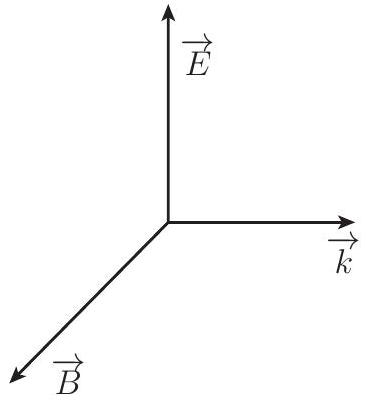
\includegraphics[width=0.7\textwidth]{images/propagation/prop-005-000.png}
\caption{Structure d'une onde plane progressive.}
\end{figure}

\begin{figure}[H]
\centering
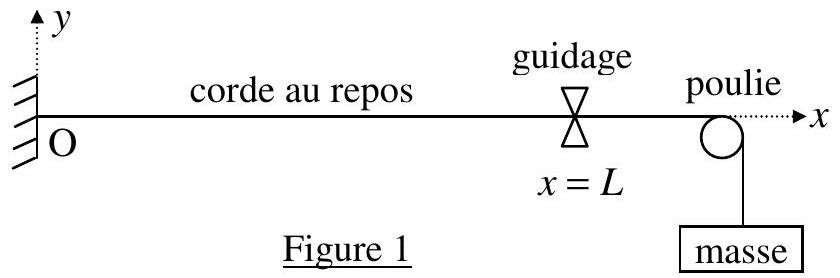
\includegraphics[width=0.7\textwidth]{images/propagation/prop-006-001.png}
\caption{Équation de propagation : schéma.}
\end{figure}

\begin{figure}[H]
\centering
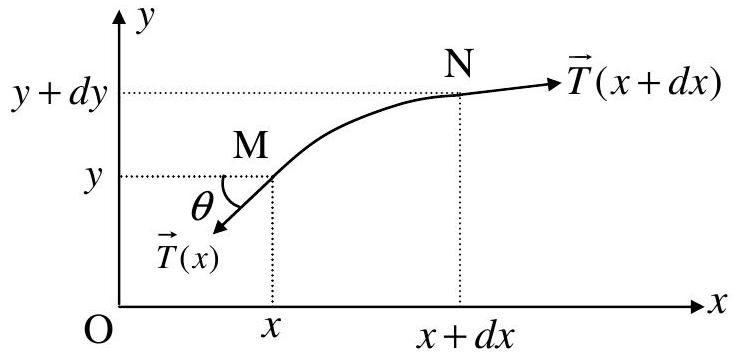
\includegraphics[width=0.7\textwidth]{images/propagation/prop-007-002.png}
\caption{Bilan énergétique d'une onde EM.}
\end{figure}

\begin{figure}[H]
\centering
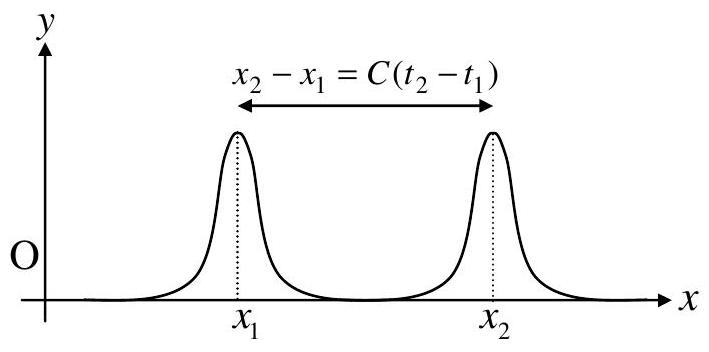
\includegraphics[width=0.7\textwidth]{images/propagation/prop-017-003.png}
\caption{Réflexion et transmission à une interface.}
\end{figure}

\begin{figure}[H]
\centering
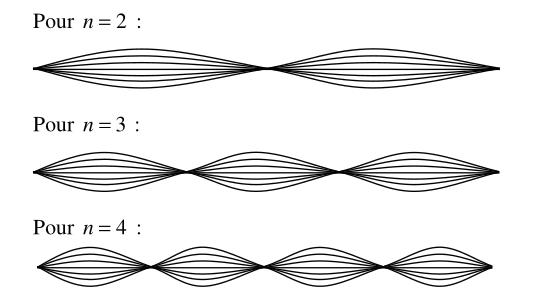
\includegraphics[width=0.7\textwidth]{images/propagation/prop-017-004.png}
\caption{Coefficients de Fresnel en incidence oblique.}
\end{figure}

\begin{figure}[H]
\centering
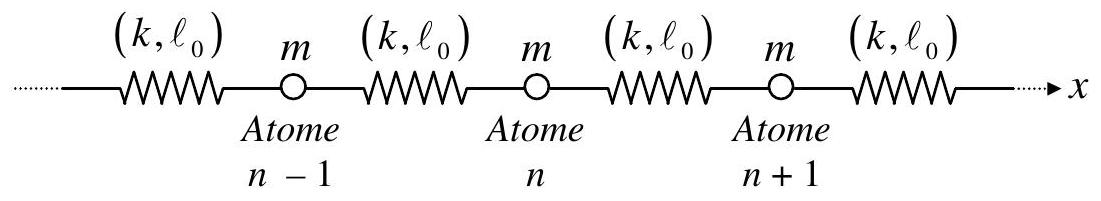
\includegraphics[width=0.7\textwidth]{images/propagation/prop-019-005.png}
\caption{Modes propres dans un milieu limité.}
\end{figure}

\begin{figure}[H]
\centering
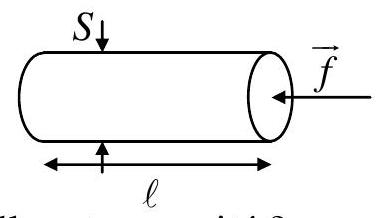
\includegraphics[width=0.7\textwidth]{images/propagation/prop-019-006.png}
\caption{Modes TE et TM dans un guide d'onde.}
\end{figure}

\begin{figure}[H]
\centering
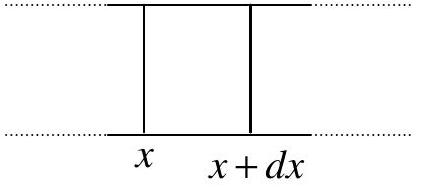
\includegraphics[width=0.7\textwidth]{images/propagation/prop-020-007.png}
\caption{Ligne de transmission : équations du télégraphiste.}
\end{figure}

\begin{figure}[H]
\centering
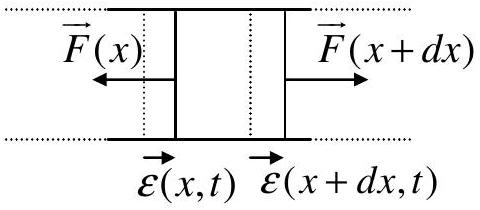
\includegraphics[width=0.7\textwidth]{images/propagation/prop-020-008.png}
\caption{Plasma : relation de dispersion.}
\end{figure}

\ifdefined\inMainDoc\else\end{document}\fi
